% !TEX root = task-1-5.tex
% Editable task bank. Append new BankTask blocks at the end of the document.
\documentclass[12pt,a4paper]{article}
\usepackage{physics-textbook}
\usepackage{graphicx,needspace}
\usetikzlibrary{decorations.pathmorphing}
\newif\ifShowSolutions
\ifdefined\TutorEdition
  \ShowSolutionstrue
\else
  \ShowSolutionsfalse % Change to \ShowSolutionstrue to display solutions.
\fi
\newcounter{banktask}
\newsavebox{\BankTaskBox}
\newcommand{\BankTaskContent}[3]{%
  \noindent\textbf{\thebanktask.}\quad #2\par
  \ifShowSolutions
    \Needspace{50mm}% Keep the solution heading with its opening text or diagram.
    #3\par
    \ifdefined\TutorEdition
      \ifcsname TutorSource#1\endcsname
        \nopagebreak\smallskip{\small\csname TutorSource#1\endcsname\par}%
      \fi
    \fi
  \fi
}
\newcommand{\BankTask}[3]{%
  \refstepcounter{banktask}\par\medskip
  \sbox{\BankTaskBox}{\begin{minipage}{\linewidth}%
    \BankTaskContent{#1}{#2}{#3}\end{minipage}}%
  \ifdim\dimexpr\ht\BankTaskBox+\dp\BankTaskBox\relax>\dimexpr\textheight-20mm\relax
    \Needspace{35mm}\BankTaskContent{#1}{#2}{#3}%
  \else
    \Needspace{\dimexpr\ht\BankTaskBox+\dp\BankTaskBox\relax}%
    \noindent\usebox{\BankTaskBox}\par
  \fi
  \medskip
}
\begin{document}
\BookSubsection{1.5}{Путь при неравномерном движении}


% Source 008243: https://ege.fipi.ru/bank/questions.php?search=1&proj=BA1F39653304A5B041B656915DC36B38&qid=008243
\BankTask{008243}{
На рисунке приведён график зависимости проекции скорости тела $\upsilon_x$ от времени $t$. Определите путь тела за первые $5$ секунд движения, в метрах.
\begin{center}
\begin{tikzpicture}[x=0.35cm,y=0.14cm,>=stealth]
\draw[black!85,thin,xstep=1,ystep=5] (0,-10) grid (20,15);
\draw[->] (0,0)--(22,0) node[right] {$t,\,\text{с}$};
\draw[->] (0,-15)--(0,19) node[above] {$\upsilon_x,\,\text{м}/\text{с}$};
\foreach \t in {5,10,15,20} \node[below] at (\t,0) {$\t$};
\foreach \v in {-10,-5,0,5,10,15} \node[left] at (0,\v) {$\v$};
\draw[very thick] (0,5)--(3,5)--(5,15)--(10,-10)--(12,-10)--(18,5)--(20,5);
\end{tikzpicture}
\end{center}
}{
\smallskip\noindent\textbf{Решение от GPT}\par
На первых $5\,\text{с}$ проекция скорости положительна. Путь равен площади под графиком:
\[
s=5\cdot3+\frac{5+15}{2}\cdot(5-3)=35\,\text{м}.
\]
}

% Source 6EC247: https://ege.fipi.ru/bank/questions.php?search=1&proj=BA1F39653304A5B041B656915DC36B38&qid=6EC247
\BankTask{6EC247}{
На рисунке представлен график зависимости модуля скорости $\upsilon$ тела от времени $t$. Найдите путь, пройденный телом за время от $0$ до $12\,\text{с}$. Результат выразите в $\text{м}$.
\begin{center}
\begin{tikzpicture}[x=0.35cm,y=0.18cm,>=stealth]
\foreach \h in {5,10,15} \draw[thin,black!65] (0,\h)--(12,\h);
\foreach \q in {2,6,8,10} \draw[thin,black!65] (\q,0)--(\q,15);
\foreach \q in {4,12} \draw[thin,dashed] (\q,0)--(\q,15);
\draw[->] (0,0)--(16,0) node[right] {$t,\,\text{с}$};
\draw[->] (0,0)--(0,20) node[above] {$\upsilon,\,\text{м}/\text{с}$};
\node[below] at (2,0) {$2$};
\node[below] at (4,0) {$4$};
\node[below] at (6,0) {$6$};
\node[below] at (8,0) {$8$};
\node[below] at (10,0) {$10$};
\node[below] at (12,0) {$12$};
\node[left] at (0,5) {$5$};
\node[left] at (0,10) {$10$};
\node[left] at (0,15) {$15$};
\draw[very thick] (0,0)--(4,15)--(12,15);
\end{tikzpicture}
\end{center}
}{
\smallskip\noindent\textbf{Решение от GPT}\par
Путь равен площади под графиком модуля скорости: $s=4\cdot15/2+(12-4)\cdot15=150\,\text{м}$.
}

% Source 41FCF3: https://ege.fipi.ru/bank/questions.php?search=1&proj=BA1F39653304A5B041B656915DC36B38&qid=41FCF3
\BankTask{41FCF3}{
На рисунке приведён график зависимости проекции $\upsilon_x$ скорости тела от времени $t$.

Определите путь, пройденный телом в интервале времени от $0$ до $5\,\text{с}$. Результат выразите в $\text{м}$.
\begin{center}
\begin{tikzpicture}[x=0.23cm,y=0.12cm,>=stealth]
\draw[thin,black!65,xstep=1,ystep=5] (0,-15) grid (20,15);
\draw[->] (0,0)--(22,0) node[right] {$t,\,\text{с}$};
\draw[->] (0,-15)--(0,20) node[above] {$\upsilon_x,\,\text{м}/\text{с}$};
\node[below] at (5,0) {$5$};
\node[below] at (10,0) {$10$};
\node[below] at (15,0) {$15$};
\node[below] at (20,0) {$20$};
\node[left] at (0,-15) {$-15$};
\node[left] at (0,-10) {$-10$};
\node[left] at (0,-5) {$-5$};
\node[left] at (0,0) {$0$};
\node[left] at (0,5) {$5$};
\node[left] at (0,10) {$10$};
\node[left] at (0,15) {$15$};
\draw[very thick] (0,15)--(5,-10)--(7,-10)--(12,5)--(15,5)--(19,-5);
\end{tikzpicture}
\end{center}
}{
\smallskip\noindent\textbf{Решение от GPT}\par
Скорость обращается в нуль при $t=3\,\text{с}$. Путь равен сумме модулей площадей: $s=15\cdot3/2+10\cdot2/2=32{,}5\,\text{м}$.
}

% Source F5e57D: https://ege.fipi.ru/bank/questions.php?search=1&proj=BA1F39653304A5B041B656915DC36B38&qid=F5e57D
\BankTask{F5e57D}{
Тело движется вдоль оси $Ox$. На рисунке приведён график зависимости проекции $\upsilon_x$ скорости тела от времени $t$.

Определите путь, пройденный телом в интервале времени от $0$ до $20\,\text{с}$. Результат выразите в $\text{м}$.
\begin{center}
\begin{tikzpicture}[x=0.12cm,y=0.12cm,>=stealth]
\draw[thin,dashed,xstep=5,ystep=5] (0,0) grid (45,25);
\draw[->] (0,0)--(50,0) node[right] {$t,\,\text{с}$};
\draw[->] (0,0)--(0,30) node[above] {$\upsilon_x,\,\text{м}/\text{с}$};
\node[below] at (10,0) {$10$};
\node[below] at (20,0) {$20$};
\node[below] at (30,0) {$30$};
\node[below] at (40,0) {$40$};
\node[left] at (0,0) {$0$};
\node[left] at (0,10) {$10$};
\node[left] at (0,20) {$20$};
\draw[very thick] (0,15)--(10,5)--(20,20)--(30,0)--(40,25);
\end{tikzpicture}
\end{center}
}{
\smallskip\noindent\textbf{Решение от GPT}\par
На интервале $0\! -\!20\,\text{с}$ скорость неотрицательна. Путь $s=(15+5)\cdot10/2+(5+20)\cdot10/2=225\,\text{м}$.
}

% Source BD0C23: https://ege.fipi.ru/bank/questions.php?search=1&proj=BA1F39653304A5B041B656915DC36B38&qid=BD0C23
\BankTask{BD0C23}{
На рисунке представлен график зависимости модуля скорости $u$ прямолинейно движущегося тела от времени $t$. Определите по графику путь, пройденный телом в интервале времени от $1$ до $5\,\text{с}$. Результат выразите в $\text{м}$.
\begin{center}
\begin{tikzpicture}[x=0.9cm,y=0.202cm,>=stealth]
\draw[thin,black!65,xstep=1,ystep=5] (0,0) grid (5,10);
\draw[->] (0,0)--(6.2,0) node[right] {$t,\,\text{с}$};
\draw[->] (0,0)--(0,15) node[above] {$\upsilon,\,\text{м}/\text{с}$};
\node[below] at (0,0) {$0$};
\node[below] at (1,0) {$1$};
\node[below] at (2,0) {$2$};
\node[below] at (3,0) {$3$};
\node[below] at (4,0) {$4$};
\node[below] at (5,0) {$5$};
\node[left] at (0,10) {$10$};
\draw[very thick] (0,0)--(1,10)--(3,10)--(5,0);
\end{tikzpicture}
\end{center}
}{
\smallskip\noindent\textbf{Решение от GPT}\par
$s=10(3-1)+10(5-3)/2=30\,\text{м}$.
}

% Source D109D1: https://ege.fipi.ru/bank/questions.php?search=1&proj=BA1F39653304A5B041B656915DC36B38&qid=D109D1
\BankTask{D109D1}{
На рисунке представлен график зависимости модуля скорости $\upsilon$ автомобиля от времени $t$. Определите по графику путь, пройденный автомобилем в интервале времени от $t_1=20\,\text{с}$ до $t_2=50\,\text{с}$. Результат выразите в $\text{м}$.
\begin{center}
\begin{tikzpicture}[x=0.09cm,y=0.21cm,>=stealth]
\draw[thin,black!65,xstep=10,ystep=5] (0,0) grid (50,10);
\draw[->] (0,0)--(70,0) node[right] {$t,\,\text{с}$};
\draw[->] (0,0)--(0,15) node[above] {$\upsilon,\,\text{м}/\text{с}$};
\node[below] at (0,0) {$0$};
\node[below] at (10,0) {$10$};
\node[below] at (20,0) {$20$};
\node[below] at (30,0) {$30$};
\node[below] at (40,0) {$40$};
\node[below] at (50,0) {$50$};
\node[left] at (0,10) {$10$};
\draw[very thick] (0,0)--(10,10)--(30,10)--(50,0);
\end{tikzpicture}
\end{center}
}{
\smallskip\noindent\textbf{Решение от GPT}\par
От $20$ до $30\,\text{с}$ путь $100\,\text{м}$, от $30$ до $50\,\text{с}$ --- $10\cdot20/2=100\,\text{м}$. Итого $s=200\,\text{м}$.
}

% Source ce6D67: https://ege.fipi.ru/bank/questions.php?search=1&proj=BA1F39653304A5B041B656915DC36B38&qid=ce6D67
\BankTask{ce6D67}{
Тело движется вдоль оси $Ox$. На рисунке приведён график зависимости проекции $\upsilon_x$ скорости тела от времени $t$.

Определите путь, пройденный телом в интервале времени от $0$ до $30\,\text{с}$. Результат выразите в $\text{м}$.
\begin{center}
\begin{tikzpicture}[x=0.12cm,y=0.12cm,>=stealth]
\draw[thin,dashed,xstep=5,ystep=5] (0,0) grid (45,25);
\draw[->] (0,0)--(50,0) node[right] {$t,\,\text{с}$};
\draw[->] (0,0)--(0,30) node[above] {$\upsilon_x,\,\text{м}/\text{с}$};
\node[below] at (10,0) {$10$};
\node[below] at (20,0) {$20$};
\node[below] at (30,0) {$30$};
\node[below] at (40,0) {$40$};
\node[left] at (0,0) {$0$};
\node[left] at (0,10) {$10$};
\node[left] at (0,20) {$20$};
\draw[very thick] (0,15)--(10,5)--(20,20)--(30,0)--(40,25)--(45,25);
\end{tikzpicture}
\end{center}
}{
\smallskip\noindent\textbf{Решение от GPT}\par
На интервале $0\! -\!30\,\text{с}$ скорость неотрицательна. Путь $s=(15+5)10/2+(5+20)10/2+20\cdot10/2=325\,\text{м}$.
}

% Source 613927: https://ege.fipi.ru/bank/questions.php?search=1&proj=BA1F39653304A5B041B656915DC36B38&qid=613927
\BankTask{613927}{
В инерциальной системе отсчёта вдоль оси $Ox$ движется тело массой $20\,\text{кг}$. На рисунке приведён график зависимости проекции $\upsilon_x$ скорости этого тела от времени $t$.
\begin{center}
\begin{tikzpicture}[x=0.05cm,y=0.6cm,>=stealth]
\draw[thin,black!65,xstep=10,ystep=1] (0,0) grid (100,4);
\draw[->] (0,0)--(120,0) node[right] {$t,\,\text{с}$};
\draw[->] (0,0)--(0,5) node[above] {$v_x,\,\text{м}/\text{с}$};
\node[below] at (0,0) {$0$};
\node[below] at (10,0) {$10$};
\node[below] at (20,0) {$20$};
\node[below] at (30,0) {$30$};
\node[below] at (40,0) {$40$};
\node[below] at (50,0) {$50$};
\node[below] at (60,0) {$60$};
\node[below] at (70,0) {$70$};
\node[below] at (80,0) {$80$};
\node[below] at (90,0) {$90$};
\node[below] at (100,0) {$100$};
\node[left] at (0,0) {$0$};
\node[left] at (0,1) {$1$};
\node[left] at (0,2) {$2$};
\node[left] at (0,3) {$3$};
\node[left] at (0,4) {$4$};
\draw[very thick] (0,0)--(30,4)--(60,4)--(90,3)--(100,0);
\end{tikzpicture}
\end{center}
\begin{enumerate}
\item В промежутке времени от $0$ до $30\,\text{с}$ проекция $\Delta x$ перемещения тела в $2$ раза меньше, чем в промежутке времени от $60$ до $90\,\text{с}$.
\item В промежутке времени от $90$ до $100\,\text{с}$ направление равнодействующей сил, действующих на тело, совпадает с направлением скорости тела.
\item В момент времени $95\,\text{с}$ проекция $F_x$ равнодействующей сил, действующих на тело, отрицательна.
\item В промежутке времени от $10$ до $30\,\text{с}$ равнодействующая сил, действующих на тело, не совершает работу.
\item Кинетическая энергия тела в момент времени $15\,\text{с}$ равна $40\,\text{Дж}$.
\end{enumerate}
}{
\smallskip\noindent\textbf{Решение от GPT}\par
При $t=95\,\text{с}$ скорость положительна, наклон отрицателен, значит $F_x=ma_x<0$. При $t=15\,\text{с}$ $v=2\,\text{м}/\text{с}$ и $E_{\text{к}}=20\cdot2^2/2=40\,\text{Дж}$. Площади за $0\! -\!30$ и $60\! -\!90\,\text{с}$ равны $60$ и $105\,\text{м}$; за $10\! -\!30\,\text{с}$ скорость растёт, поэтому работа положительна. Ответ: $35$.
}

% Source E74C4C: https://ege.fipi.ru/bank/questions.php?search=1&proj=BA1F39653304A5B041B656915DC36B38&qid=E74C4C
\BankTask{E74C4C}{
Учащиеся роняли с башни шарики для настольного тенниса и снимали их полёт цифровой видеокамерой. Обработка видеозаписей позволила построить графики зависимости пути $s$, пройденного шариком, и его скорости $v$ от времени падения $t$.
\begin{center}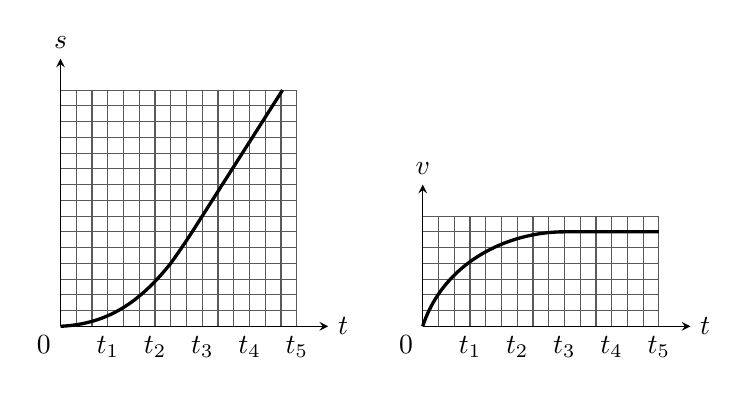
\begin{tikzpicture}[x=.2cm,y=.2cm,>=stealth]
\draw[thin,black!65,step=1] (0,0) grid (15,15);
\draw[->] (0,0)--(17,0) node[right] {$t$};\draw[->] (0,0)--(0,17) node[above] {$s$};
\node[below left] at (0,0) {$0$};
\foreach \x/\i in {3/1,6/2,9/3,12/4,15/5} \node[below] at (\x,0) {$t_{\i}$};
\draw[very thick] (0,0) .. controls (3,.15) and (5,1.5) .. (7,4) .. controls (8,5.4) and (8.49,6.2) .. (9,7) --(14.1,15);
\begin{scope}[xshift=4.6cm]
\draw[thin,black!65,step=1] (0,0) grid (15,7);
\draw[->] (0,0)--(17,0) node[right] {$t$};\draw[->] (0,0)--(0,9) node[above] {$v$};
\node[below left] at (0,0) {$0$};
\foreach \x/\i in {3/1,6/2,9/3,12/4,15/5} \node[below] at (\x,0) {$t_{\i}$};
\draw[very thick] (0,0) .. controls (1.3,4) and (5.3,6) .. (9,6) --(15,6);
\end{scope}\end{tikzpicture}\end{center}
\begin{enumerate}
\item В течение всего времени падения ($0$ — $t_{5}$) потенциальная энергия шарика в поле тяжести, отсчитываемая от основания башни, уменьшалась.
\item В течение всего времени падения ($0$ — $t_{5}$) величина импульса шарика постоянно возрастала.
\item Величина ускорения, с которым падал шарик, уменьшалась в интервале времени ($0$ — $t_{3}$).
\item Величина ускорения, с которым падал шарик, увеличивалась в интервале времени ($0$ — $t_{3}$) и оставалась постоянной при $t>t_{4}$.
\item Сумма кинетической и потенциальной энергий шарика оставалась неизменной во время падения.
\end{enumerate}
}{
\smallskip\noindent\textbf{Решение от GPT}\par
Шарик всё время опускается: $E_{\text{п}}=mgh$ уменьшается. Наклон графика $v(t)$ до $t_3$ уменьшается, значит ускорение уменьшается. Затем скорость и импульс постоянны. Сопротивление воздуха совершает отрицательную работу, поэтому механическая энергия не сохраняется. Ответ: $13$.
}

\end{document}
